\chapter{The Model}

\section{Hamiltonian 1}

This is a Hamiltonian for an odd-mass triaxial nucleus:
\begin{align}
    \hat{H}=\hat{H}_\text{core}+\hat{H}_\text{s.p.}
\end{align}

The PRM Hamiltonian was firstly described in a quantal approach by Davydov and Filippov \cite{davydov1958rotational}. The calculations from \cite{bohr1998nuclear} gave predictions on the \textbf{wobbling motion}.
\begin{figure}[ht]
    \centering
    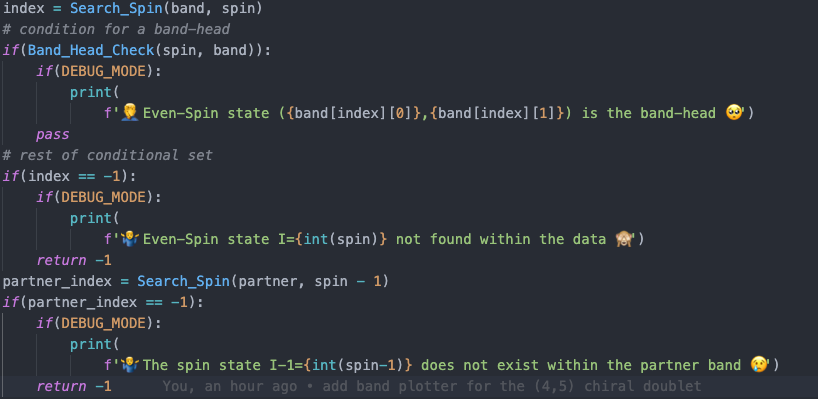
\includegraphics[width=0.85\textwidth]{figs/cuterr_code.png}
    \caption{My GitHub Account.}
    \label{github_account}
\end{figure}
\begin{figure}[ht]
    \centering
    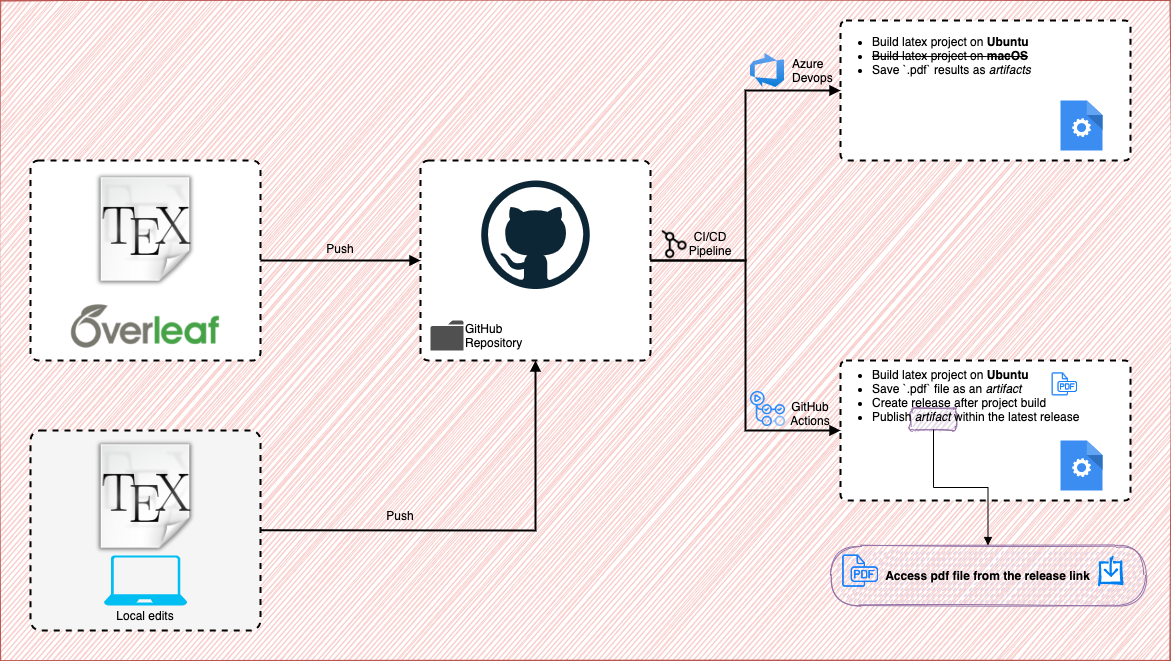
\includegraphics[width=0.97\textwidth]{figs/overleaf-book.png}
    \caption{The \texttt{CI/CD} workflow.}
    \label{workflow-scheme}
\end{figure}

Figures \ref{github_account} and \ref{workflow-scheme} represent the potential work done in \cite{poenaru2021parity}.

\lipsum[1-3]
    
